\section{Simulations}

\subsection{Numerical implementation}

\subsubsection{Evolution equation}

Starting from \autoref{eq:eq1}, we want to obtain an equation to numerically calculate the wave height at the next timestep \(t_{i+1}\) using the previous heights at positions \(x_i\), \(x_{i-1}\) and \(x_{i+1}\). Using the following approximations for the derivatives
\begin{equation}
    \frac{\partial F}{\partial x}(x_i) \approx \frac{F(x_{i+1}) - F(x_{i-1})}{2 \Delta x}
    , \qquad
    \frac{\partial^2 F}{\partial x^2}(x_i) \approx \frac{F(x_{i+1}) - 2 F(x_i) + F(x_{i-1})}{(\Delta x)^2}
\end{equation}
where \(F\) is a generic function representing either \(f\) or \(h_0\), \(\Delta x = x_{i+1} - x_i\) as the mesh is regular and \(x\) is a generic variable representing either \(x\) or \(t\). \autoref{eq:eq1} is equivalent to:
\begin{equation}
    \frac{\partial^2 f}{\partial t^2} = g \frac{\partial h_0}{\partial x} \frac{\partial f}{\partial x} + g h_0 \frac{\partial^2 f}{\partial x^2}
\end{equation}
Then using the previously mentioned formulas:
\begin{equation}
    \begin{aligned}
        \frac{f(x_i, t_{i+1}) - 2 f(x_i, t_i) + f(x_i, t_{i-1})}{(\Delta t)^2} &= g \left( \frac{h_0(x_{i+1}) - h_0(x_{i-1})}{2 \Delta x} \right) \left( \frac{f(x_{i+1}, t_i) - f(x_{i-1}, t_i)}{2 \Delta x} \right) \\
        &+ g h_0(x_i) \frac{f(x_{i+1}, t_i) - 2 f(x_i, t_i) + f(x_{i-1}, t_i)}{(\Delta x)^2}
    \end{aligned}
\end{equation}
By rearanging and identifying the Courant-Friedrichs-Lewy constant \(\beta(x) = u(x) \frac{\Delta t}{\Delta x} = \sqrt{g h_0(x)} \frac{\Delta t}{\Delta x}\) we get the following equation:
\begin{equation}
    \begin{aligned}
        f(x_i, t_{i+1}) &= \frac{1}{4} \left( \beta(x_{i+1})^2 - \beta(x_{i-1})^2 \right) \left( f(x_{i+1}, t_i) - f(x_{i-1}, t_i) \right) \\
        &+ \beta(x_i)^2 (f(x_{i+1}, t_i) - 2 f(x_i, t_i) + f(x_{i-1}, t_i)) \\
        &+ 2 f(x_i,t_i) \\
        &- f(x_i,t_{i-1})
    \end{aligned}
\end{equation}
The evolution for \autoref{eq:eq2} is taken from \cite{physnumbook}, equation 4.43.

\subsubsection{Border conditions}

The simulation implements border conditions for a fixed border (the wave has a specific height at the border), a free border (the wave is allowed to move as it pleases along the border) and an exit condition (the wave continues as if there was no border). These conditions are given in the numerical physics book \cite{physnumbook} (section 4.2.1), for the left and right borders for exit and free borders as well as the exit condition for the right border. We will derive the exit conditions for the left border here. Under this condition, the left border only has a retrograde wave, i.e. \(f(x, t) = f_+(x + u t)\). Differentiating w.r.t. to \(t\) and \(x\), at \(x = x_L\) (left border) we obtain the following relationship:
\begin{gather}
    \frac{\partial f}{\partial t}(x_L, t) = \frac{\partial f_+(x_L + u t)}{\partial t} = u f_+'(x_L + u t) \\
    \frac{\partial f}{\partial x}(x_L, t) = f_+'(x_L + u t) \\
    \implies \frac{\partial f}{\partial t}(x_L, t) = u \frac{\partial f}{\partial x}(x_L, t)
\end{gather}
Discretising using the "forward" finite difference method, i.e. \(\frac{\partial F(x_i)}{\partial x} \approx (F(x_{i+1}) - F(x_i))/\Delta x\), for both time and space derivatives, and identifying \(x_L \equiv x_0\) the first position in the discretised list, we get:
\begin{equation}
    \frac{f(x_0,t_{n+1}) - f(x_0, t_n)}{\Delta t} = u \frac{f(x_1, t_n) - f(x_0, t_n)}{\Delta x}
\end{equation}
Rearanging and identifying the CFL constant we then get:
\begin{equation}
    f(x_0, t_{n+1}) = f(x_0, t_n) + \beta \left( f(x_1, t_n) - f(x_0, t_n) \right)
\end{equation}

\subsubsection{Initial conditions}

The initial conditions for a left and right moving wave, as well as a static wave were implemented using equations 4.48 to 4.50 given in \cite{physnumbook}.

The initial position and height of the wave can be chosen to be either:
\begin{equation}
    f_\textrm{init}(x) = \begin{cases}
        \begin{aligned}
            &0 &&(x \le x_1)\\
            & {\frac{A}{2} \left( 1 - \cos \left( 2\pi\frac{x-x_1}{x_2-x_1} \right) \right)} &&(x_1 < x < x_2)\\
            &0 &&(x_2 \le x)
        \end{aligned}
    \end{cases}
    \label{eq:form_init}
\end{equation}
or initialised in normal modes according to \autoref{eq:normal_initial}.




\subsection{Wave with constant velocity}
In this first simulation we consider a basin going from $x_L = 0$ \si{\meter} to $x_R = 10$ \si{\meter}. The water inside of it has a constant depth of $h_0 = 3$ \si{\meter}. The left border of the water is fixed and the right side is free. 

\paragraph{Reflecting waves} We first want to analyse reflecting waves in the basin. For this we simulate the behavior of a wave initialised according to \autoref{eq:form_init} with $A = 1$ \si{\meter}, $x_1 = 2$ \si{\meter} and $x_2 = 6$ \si{\meter}. It is given initial velocities to the left and to the right and no initial velocity in three different simulations. It is each time simulated until the time $t_\mathrm{fin}$ for two round trips across the basin, i.e. $t_\mathrm{fin} = 4L/u$ with $L = x_R - x_L = 10$ \si{\meter} the length of the basin and $u = \sqrt{gh_0}$ the speed of the wave in the basin. The results of these simulations are shown in \autoref{fig:basin_movements}.
\begin{figure}[h]
    \centering
    \begin{subfigure}{0.48\linewidth}
        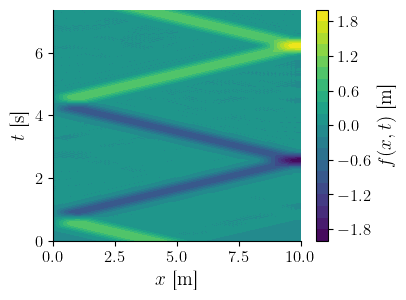
\includegraphics[width=\linewidth]{figures/bassin_default_left.png}
        \caption{Oriented left}
        \label{fig:basin_left}
    \end{subfigure}
    \begin{subfigure}{0.48\linewidth}
        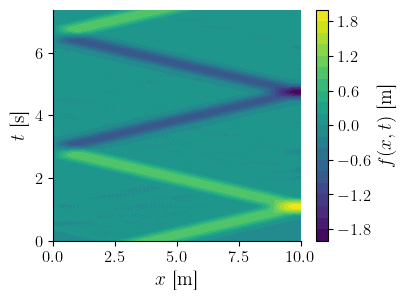
\includegraphics[width=\linewidth]{figures/bassin_default_right.png}
        \caption{Oriented right}
        \label{fig:basin_right}
    \end{subfigure}
    \begin{subfigure}{0.48\linewidth}
        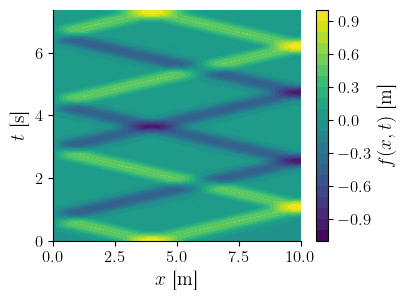
\includegraphics[width=\linewidth]{figures/bassin_default_static.png}
        \caption{With no initial orientation}
        \label{fig:basin_static}
    \end{subfigure}
    \caption{Propagation of a wave in a basin with various initial velocities}
    \label{fig:basin_movements}
\end{figure}

It is possible to observe the expected behaviors for moving waves in \autoref{fig:basin_left} and \autoref{fig:basin_right} with respectively the peak of the wave moving to the left of the basin $x_L = 0$ \si{\meter} and to the right $x_R = 10$ \si{\meter} at the beginning of the simulation. The initial behavior of the wave with no initial velocity is of two waves of opposite directions. This shows that a wave of velocity 0 \si{\meter\per\second} can be created from two opposing waves of half the amplitude. It is also noted that all the waves in these figures come back to their exact starting position and orientation of the velocity at the end of the simulation. This shows that waves in this basin go on in a periodic movement of period $t_\mathrm{fin}$ which corresponds to two round trips at speed $u$.

When it comes to the behavior of these waves in the reflection they all behave the same and this behavior depends on the type of condition placed on the border as observed in the three figures of \autoref{fig:basin_movements}. As expected the fixed condition on the left nullifies and then reverts the wave and it has negative amplitude $-A$ when it goes back to the right. The free condition gives a peak of twice the amplitude and then reflects the wave with the same sign of $A$ but with velocity to the left. A final point of interest is that \autoref{fig:basin_static} shows well the principle of superposition emerging from the linearity of \autoref{eq:eq1}. The waves do amplify or counteract each other when close but then go on in the same way as if they add not encountered each other.


\paragraph{Stability depending on CFL} The simulation has displayed the expected behavior however it can be interesting to check its stability and especially around the value of the CFL $\beta = 1$. Indeed according to the known theory, \cite{physnumbook} in section 4.2.2, this method is stable for $|\beta| \leq 1$. The first step was to check a few values of $\beta$ to get a empiric view on this. Four values of $\beta$ around 1 are shown in \autoref{fig:CFL_empiric}.
\begin{figure}[h]
    \centering
    \begin{subfigure}{0.48\linewidth}
        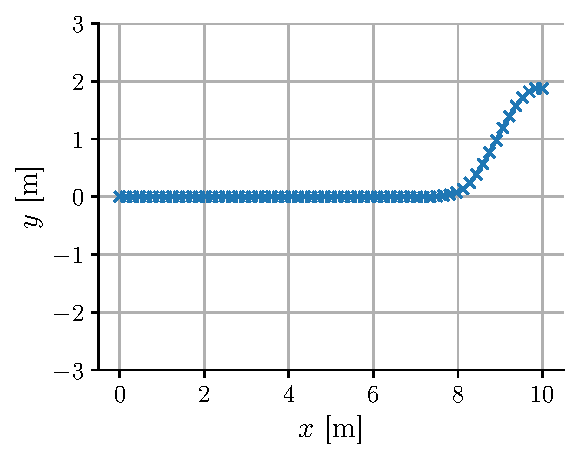
\includegraphics[width=\linewidth]{figures/bassin_default_CFL0.5_1.15s.pdf}
        \caption{$\beta = 0.5$}
        \label{fig:CFL_0.5}
    \end{subfigure}
    \begin{subfigure}{0.48\linewidth}
        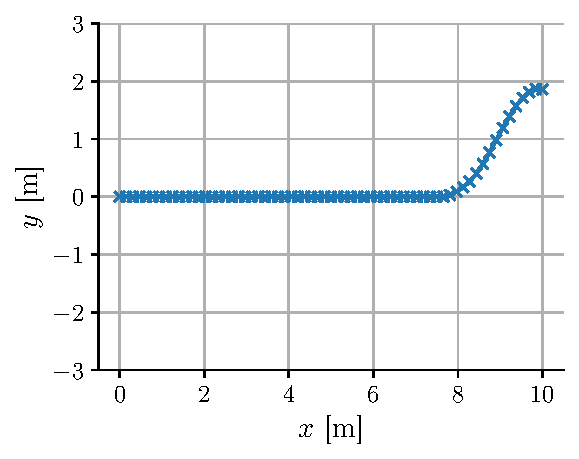
\includegraphics[width=\linewidth]{figures/bassin_default_CFL1_1.15s.pdf}
        \caption{$\beta = 1$}
        \label{fig:CFL_1}
    \end{subfigure}
    \begin{subfigure}{0.48\linewidth}
        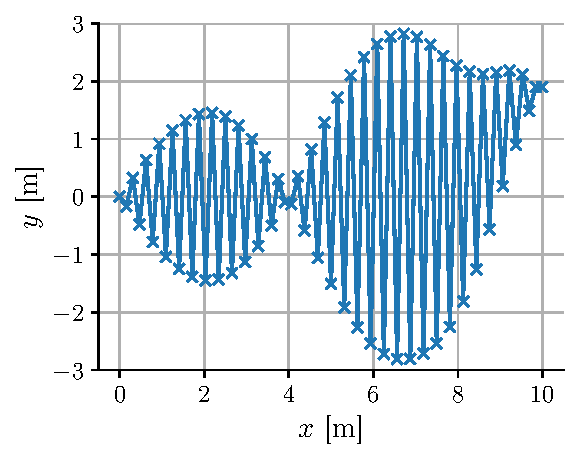
\includegraphics[width=\linewidth]{figures/bassin_default_CFL1.01_1.15s.pdf}
        \caption{$\beta = 1.01$}
        \label{fig:CFL_1.01}
    \end{subfigure}
    \begin{subfigure}{0.48\linewidth}
        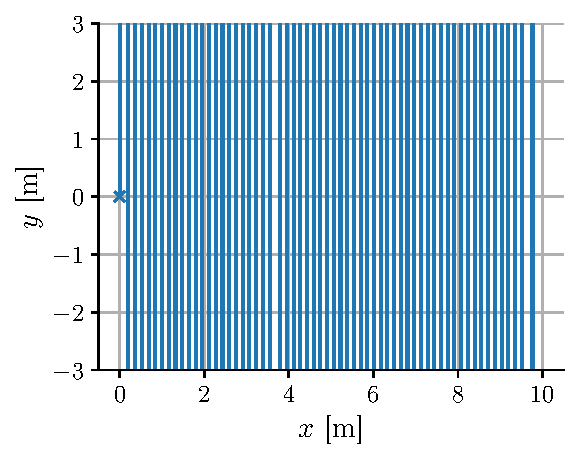
\includegraphics[width=\linewidth]{figures/bassin_default_CFL1.5_1.15s.pdf}
        \caption{$\beta = 1.5$}
        \label{fig:CFL_1.5}
    \end{subfigure}
    \caption{Simulations of a wave in a basin up to 1.15 \si{\second} for different values of the CFL}
    \label{fig:CFL_empiric}
\end{figure}

This looks a lot like a numerical instability but to be fully rigorous we need to show that it diverges exponentially from the expected behavior. For this we take back the situation where $\beta = 1.01$ as it seems to have diverged but we are not sure if it is unstable by this definition. The \autoref{fig:CFL_exp} shows the maximum amplitude of the simulation according to time that should remain between a factor 2 of the start, as the reflection on the free side gives a doubled amplitude during the reflection. We see however a line in this semi-logarithmic scale indicating that the value of the maximum amplitude grow exponentially. This is according to our definition and we can thus say that this divergence is a nulerical instability.
\begin{figure}
    \centering
    \begin{subfigure}{0.48\linewidth}
        \centering
        \includegraphics*[width=\linewidth]{figures/bassin_default_CFL_exponential.pdf}
        \caption{Over time for CFL $\beta = 1.01$}
        \label{fig:CFL_exp}
    \end{subfigure}
    \begin{subfigure}{0.48\linewidth}
        \centering
        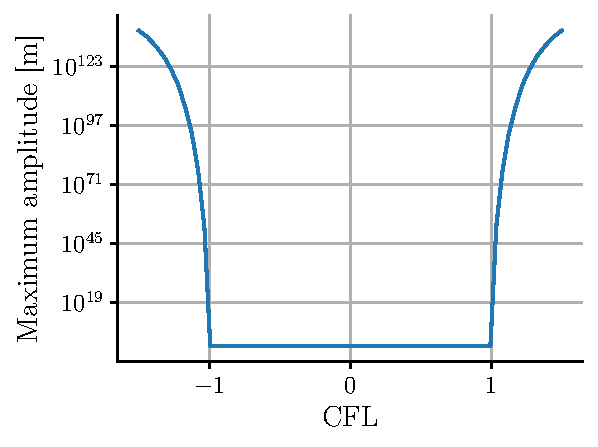
\includegraphics[width=\linewidth]{figures/bassin_default_CFL_stability.pdf}
        \caption{At the end of the simulation lasting one analytical period $t_\mathrm{fin}$ as a function of the CFL}
        \label{fig:CFL_stable}
    \end{subfigure}
    \caption{Maximum amplitude of a simulated wave in a basin. Using \(n_x=64\) intervals.}
\end{figure}


The difference between \autoref{fig:CFL_1} and \autoref{fig:CFL_1.01} clearly seems to indicate that the stability lies at $\beta = 1$. We can check this by running simulations for numerous values of $\beta$ around 1 with always the same number of intervals in the position grid in order not to influence this stability study. This was done for 100 values of $\beta$ between -1.2 and 1.2 and the result is shown in \autoref{fig:CFL_stable}.

The \autoref{fig:CFL_stable} clearly shows the difference between the domain $|\beta| \leq 1$ and $|\beta| > 1$. We thus verified that the condition for stability in this simulation is $|\beta| \leq 1$ which is in line with the theory.


\paragraph{Normal modes} The final simulation run for this basin is a study of its normal modes. Indeed with these border conditions it is possible to calculate the normal modes to have stationary waves as done in \autoref{sec:normal_modes}. We then want to simulate a wave starting as in \autoref{eq:normal_initial} to verify if our simulation does show the behavior of a stationary wave. Using \autoref{eq:normal_initial} with $A = 0.5$ \si{\meter} and $n = 2$ the number of the normal mode we initialised our simulation as shown in \autoref{fig:normal_init}.
\begin{figure}[h]
    \centering
    \includegraphics*[width=0.6\linewidth]{figures/bassin_mode_start.pdf}
    \caption{Initialisation of the normal mode}
    \label{fig:normal_init}
\end{figure}

The simulation was run until the end of one period of the stationary wave as calculated analytically, using \autoref{eq:normal_frequency} we have one period:
\begin{equation}
    t_\mathrm{fin} = T_n = \frac{1}{\nu_n} = \frac{4(x_R - x_L)\sqrt{gh_0}}{2n + 1}
\end{equation}
The simulation was run for a value of the CFL $\beta = 1$ and various values of the number of intervals $n_x$. This gave a value for $\Delta x$ knowing the length of the basin $L$ and thus a value for $\Delta t$ knowing $\beta = u\Delta t/\Delta x$. The result of the simulation for the greatest number of intervals (and thus the most precise) is given in \autoref{fig:normal_level}. We can observe that the number of the normal mode $n$ corresponds to the number of nodes or peaks when not considering the borders.

\begin{figure}[h]
    \begin{minipage}{0.48\linewidth}
        \centering
        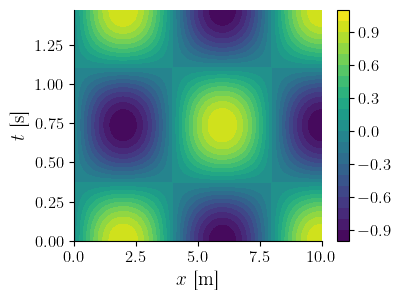
\includegraphics[width=\linewidth]{figures/bassin_mode_level.png}
        \captionof{figure}{Simulation of a normal mode of a basin with CFL = 1 and $n_x = 5120$ intervals in the position mesh}
        \label{fig:normal_level}
    \end{minipage}
    \hspace*{0.4cm}
    \begin{minipage}{0.48\linewidth}
        \centering
        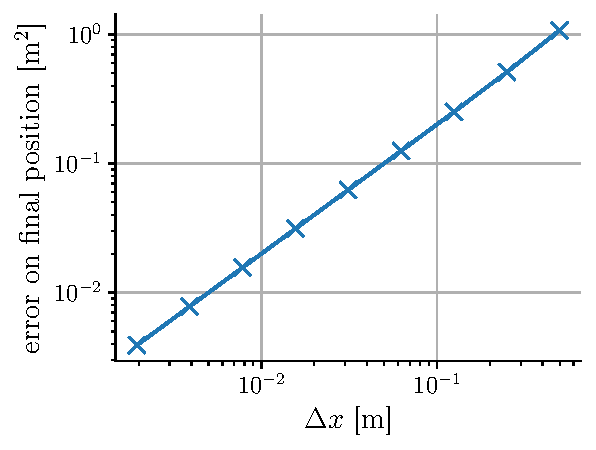
\includegraphics[width=\linewidth]{figures/bassin_mode_convergence.pdf}
        \captionof{figure}{Convergence of a simulation for a normal mode of a wave at CFL constant $\beta = 1$}
        \label{fig:normal_convergence}
    \end{minipage}
\end{figure}

It is observed in \autoref{fig:normal_level} that the simulation seems to behave as expected with a return to the original position after one analytical period, at least for a large value of $n_x$. It is therefore interesting to do a convergence analysis on these simulations according to $n_x$ or equivalently to the size of the intervals $\Delta x$. We want to keep the CFL constant at $\beta \equiv 1$ to not influence our study with changes in the simulation. We have:
\begin{equation}
    \beta = 1 = u\frac{\Delta t}{\Delta x} = u \frac{t_\mathrm{fin}}{n_{\textrm{steps}}}\frac{n_x}{L}
\end{equation}
with $n_\mathrm{steps}$ the number of steps in the time evolution. We then want to increase $n_x$ by multiplying it and to keep $\beta$ constant multiply $n_\mathrm{steps}$ by the same factor. This was done with power of 2 from 0 to 8. Knowing that the simulation should converge to the analytical solution we calculated an error $\varepsilon$ using the formula:
\begin{equation}
    \varepsilon = \int_{x_L}^{x_R} |f_\mathrm{num}(x, t=t_\mathrm{fin}) - f_\mathrm{ana}(x, t=t_\mathrm{fin})|\mathrm{d}x
\end{equation}
with $f_\mathrm{num}$ the results of the simulation and $f_\mathrm{ana}$ the analytical function given in \autoref{eq:normal_mode_explicit}. This integral was discretised to be calculated using the output of the simulation. The resulting convergence analysis is shown in \autoref{fig:normal_convergence}.
% \begin{figure}[h]
%     \centering
%     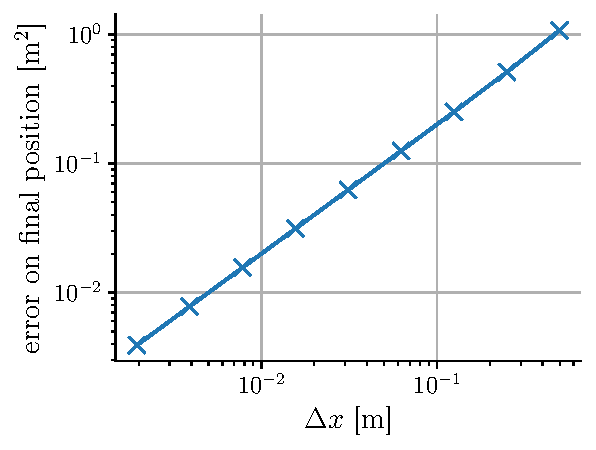
\includegraphics[width=0.6\linewidth]{figures/bassin_mode_convergence.pdf}
%     \caption{Convergence of a simulation for a normal mode of a wave at CFL constant $\beta = 1$}
%     \label{fig:normal_convergence}
% \end{figure}

We thus find that the simulation does converge to the analytical solution as the error $\varepsilon$ tends to 0 as $\Delta x$ tends to 0. However the order of convergence is of only 1 which indicates that this simulation requires a lot of computation if precise results are needed.

\subsection{Oceanic wave on a coral reef}

In this section we will use the following function for oceanic depth:
\begin{equation}
    h_0(x) = \begin{cases}
        \begin{aligned}
            &h_L &&(x_L \le x \le x_a) \\
            &\frac{1}{2}(h_L + h_C) + \frac{1}{2}(h_L - h_C) \cos \left( \pi \frac{x-x_a}{x_b-x_a} \right) &&(x_a < x < x_b) \\
            &h_C &&(x_b \le x \le x_c) \\
            &\frac{1}{2}(h_R + h_C) - \frac{1}{2}(h_R - h_C) \cos \left( \pi \frac{x-x_c}{x_d-x_c} \right) &&(x_c < x < x_d) \\
            &h_R &&(x_d \le x \le x_R)
        \end{aligned}
    \end{cases}
\end{equation}
We will choose \(h_L = 7000\)m, \(h_C = 35\)m, \(h_R = 200\)m, \(x_L = 0\)m, \(x_a = 300\)km, \(x_b = 700\)km, \(x_c = 720\)km, \(x_d = 850\)km and \(x_R = 1000\)km. The initial conditions will be a right moving wave with \(x_1 = 50\)km, \(x_2 = 250\)km and amplitude \(A = 1\)m. Both border conditions will be set to exit, to be more representative of an actual large ocean. The simulations were done until the wave passes the coral reef entirely, which corresponds to a time of about \(t = 12000\) \si{\second}. The timestep \(\Delta t\) was chosen such that \(\max(\beta_{\textrm{CFL}}) = 1\), which is \(\Delta t = \Delta x / \max_x(u(x)^2)\). The number of intervals was chosen to be 8192.

\paragraph{Simple wave} \autoref{fig:corail_eq1_mouv} shows the obtained wave motion when using \autoref{eq:eq1}. The depth profile of the water is shown in \autoref{fig:corail_eq1_depth}. We can see that around \(x=600\)km, the wave slows down considerably with a peak in amplitude, which corresponds to when the wave is right above the reef. We will study the amplitude and speed later. The observed behavior makes sense intuitively, as a wave would indeed get larger when the water becomes less deep.

\begin{figure}[h]
    \centering
    \begin{subfigure}{0.53\linewidth}
        \centering
        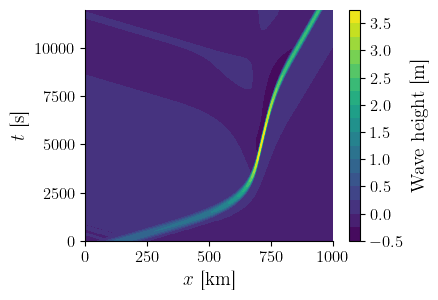
\includegraphics[width=\linewidth]{figures/corail_eq1_mouvement_vague.png}
        \caption{Wave function}
        \label{fig:corail_eq1_mouv}
    \end{subfigure}
    \begin{subfigure}{0.46\linewidth}
        \centering
        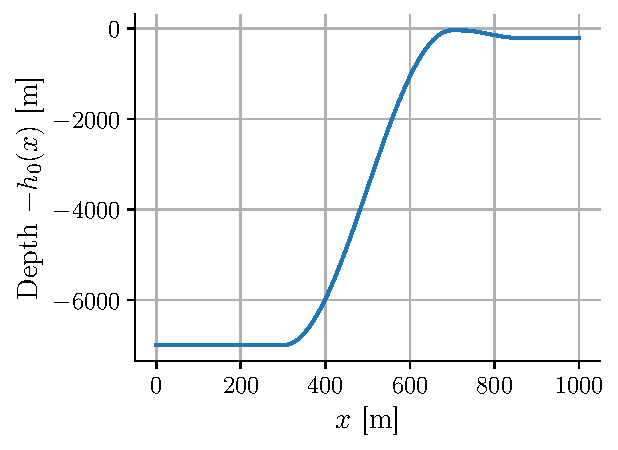
\includegraphics[width=\linewidth]{figures/corail_eq1_depth.pdf}
        \caption{Depth profile}
        \label{fig:corail_eq1_depth}
    \end{subfigure}
    \caption{Wave height as a function of space and time and depth profile. Simulated using \(n=8192\) intervals, until \(t=12000\) \si{\second}. CFL \(\beta=1\)}
\end{figure}

The maximum amplitude of the wave was obtained using a quadratic fit for every point around the time of its maximum amplitude. The maximum of the fit gave the maximum amplitude. Results are shown in \autoref{fig:corail_eq1_amplitude}. The simulation shows that the maximum amplitude increases up to the point of the coral reef, remains more or less constant on top of the reef and then goes back down. The peak amplitude above the reef (\(x_b < x < x_c\)) was found to be about 3.58m, while after the reef (\(x_d<x<x_R\)) the maximum amplitude was 2.30m. When compared to the WKB solution of \autoref{eq:eq1} given in \cite{physnumbook} (section 4.2.4), we notice that the amplitude is a bit lower than expected on top and after the reef, while it matches almost exactly before the reef. This discrepency can be attributed to either numerical imprecision or the effect of higher order terms.

Using the analysis done on the amplitude, the speed of the peak of the wave was calculated using the time \(t_{\textrm{peak},i}\) at which the fitted function is maximal. Then for every point \(x_i\), except for border cases, the speed is given by \(v_i = (x_{i+k} - x_{i-k})/(t_{\textrm{peak},i+k} - t_{\textrm{peak},i-k})\), where \(k\) is chosen such that the oscillations in \(v\) are minimal. The results are shown in \autoref{fig:corail_eq1_vitesse}. We can see that the speed decreases drastically between the starting position of the wave and the coral reef, by a factor of about 11: the speed above the reef was found to be 18 m/s, while the initial speed was 261 m/s. After the reef, the speed increases again to around 42 m/s. The simulation matches the WKB solution exactly since the speed is calculated using the same formula for both.

\begin{figure}[h]
    \centering
    \begin{subfigure}{0.48\linewidth}
        \centering
        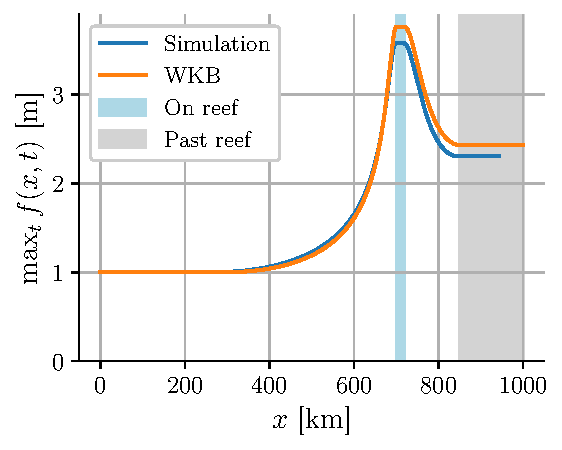
\includegraphics[width=\linewidth]{figures/corail_eq1_amplitude_wkb.pdf}
        \caption{Maximum amplitude reached at each position}
        \label{fig:corail_eq1_amplitude}
    \end{subfigure}
    \begin{subfigure}{0.48\linewidth}
        \centering
        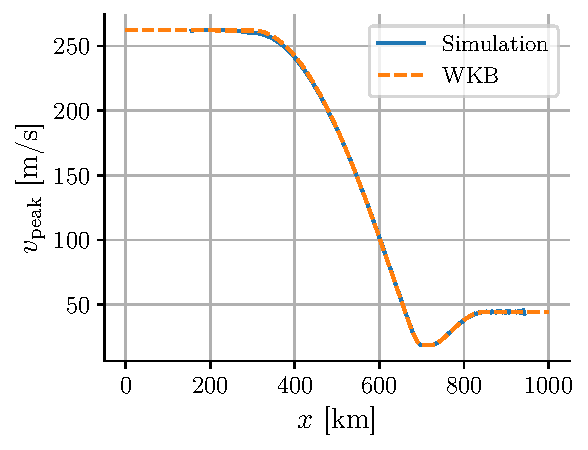
\includegraphics[width=\linewidth]{figures/corail_eq1_vitesse_wkb.pdf}
        \caption{Speed of wave peak}
        \label{fig:corail_eq1_vitesse}
    \end{subfigure}
    \caption{Properties of the wave going towards the coral reef, compared to WKB solution. Simulated using \(n=8192\) intervals, until \(t=12000\). CFL \(\beta=1\)}
    \label{fig:corail_eq1_properties}
\end{figure}

\paragraph{Steep coral reef} We would now like to analyse what happens when the slope becomes really steep, by setting \(x_a\) closer and closer to \(x_b\). Here we chose to look at the cases

where the distance between \(x_b\) and \(x_a\) was 100km and 50km, as the 400km case was treated previously. \autoref{fig:corail_eq1_mouv_xa=60km} and \autoref{fig:corail_eq1_mouv_xa=65km} show the obtained wave function. The depth profile for both cases is also shown in \autoref{fig:corail_eq1_depth_xa}. We notice an interesting phenomenon: as the slope becomes steeper, a large part of the wave gets reflected at the reef. This is similar to a change in medium, with different density, leading to a greater reflected wave and a smaller transmitted one.

\begin{figure}[h]
    \centering
    \begin{subfigure}{0.48\linewidth}
        \centering
        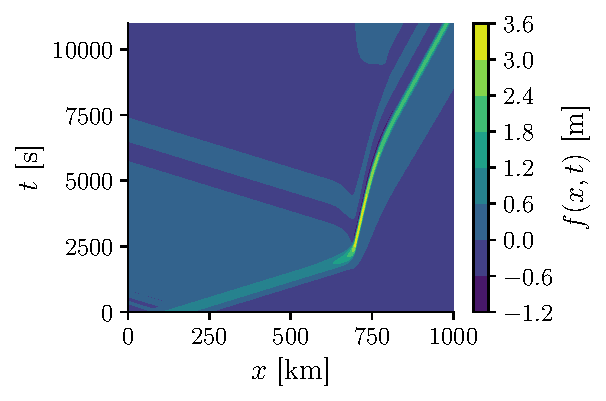
\includegraphics[width=\linewidth]{figures/corail_eq1_movement_xa=600000.pdf}
        \caption{\(x_a = 600\)km}
        \label{fig:corail_eq1_mouv_xa=60km}
    \end{subfigure}
    \begin{subfigure}{0.48\linewidth}
        \centering
        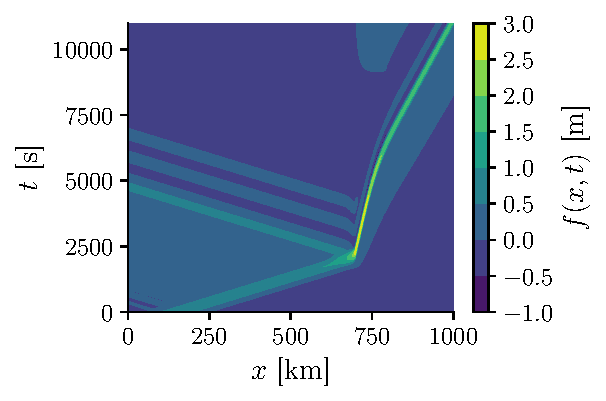
\includegraphics[width=\linewidth]{figures/corail_eq1_movement_xa=650000.pdf}
        \caption{\(x_a = 650\)km}
        \label{fig:corail_eq1_mouv_xa=65km}
    \end{subfigure}
    \caption{Wave height as a function of space and time. Simulated using \(n=8192\) intervals until \(t=12000\). CFL \(\beta=1\)}
    \label{fig:corail_eq1_mouv_xa}
\end{figure}

\begin{wrapfigure}{R}{0.5\linewidth}
    \vspace*{-0.8cm}
    \centering
    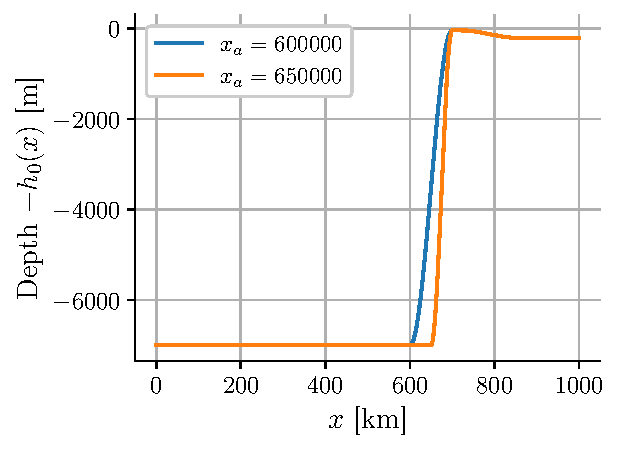
\includegraphics[width=\linewidth]{figures/corail_eq1_depth_var_xa.pdf}
    \caption{Depth profile for different \(x_a\)}
    \label{fig:corail_eq1_depth_xa}
    \vspace*{-0.4cm}
\end{wrapfigure}
Using the same analysis methods as before, we obtain the amplitude in \autoref{fig:corail_eq1_amplitude_xa=60km} and \autoref{fig:corail_eq1_amplitude_xa=65km}. We notice that as the slope gets steeper, the simulated wave becomes less and less high when on the reef. Compared to the WKB solution, the simulation severely undershoots, with a difference of about 1m on and after the reef for \(x_a = 650\)km. This difference can be attributed by the fact that WKB suppose a reasonably small change in depth, while this change of about 7000m over 50km could be considered "too fast". For the speed of the wave, the \autoref{fig:corail_eq1_speed_xa=60km} and \autoref{fig:corail_eq1_speed_xa=65km}, we notice that the simulations follows the WKB solution closely, except when near the cliff, with the effect being more important for \(x_a = 650\)km. This effect does not seem physical and could be attributed to numerical effects: if we consider a vertical slope, the wave would travel across an interface between to "mediums" with different propagation speeds, the speed would only change rapidly at the interface and not before.

\begin{figure}[H]
    \centering
    \begin{subfigure}{0.48\linewidth}
        \centering
        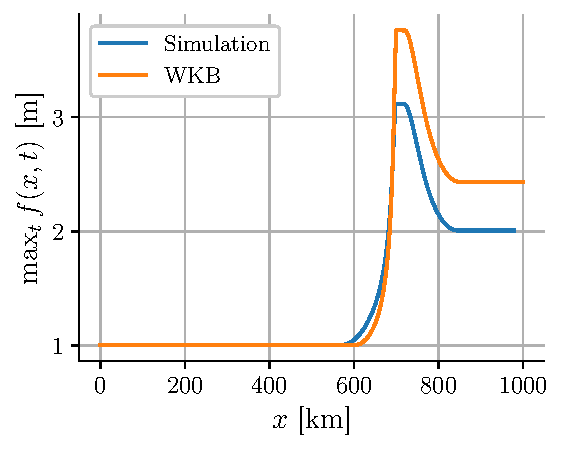
\includegraphics[width=\linewidth]{figures/corail_eq1_amplitude_xa=600000.0.pdf}
        \caption{Maximum amplitude}
        \label{fig:corail_eq1_amplitude_xa=60km}
    \end{subfigure}
    \begin{subfigure}{0.48\linewidth}
        \centering
        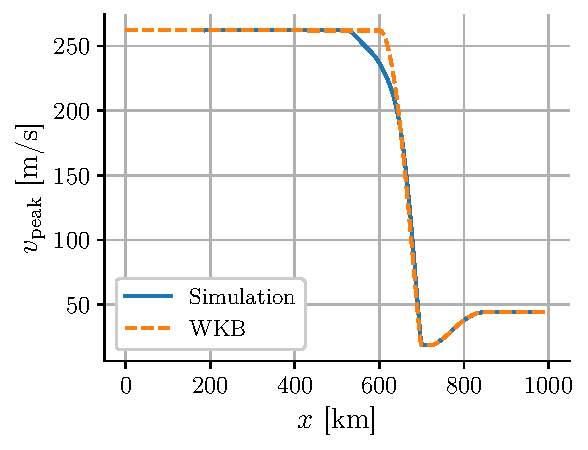
\includegraphics[width=\linewidth]{figures/corail_eq1_vitesse_xa=600000.0.pdf}
        \caption{\(x_a = 600\)km}
        \label{fig:corail_eq1_speed_xa=60km}
    \end{subfigure}
    \caption{Wave properties for \(x_a = 60\)km. Simulated using \(n=8192\) intervals until \(t=12000\). CFL \(\beta=1\)}
\end{figure}

\begin{figure}[H]
    \centering
    \begin{subfigure}{0.48\linewidth}
        \centering
        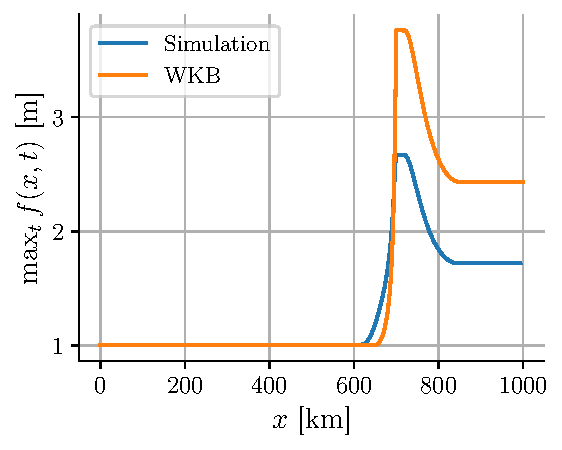
\includegraphics[width=\linewidth]{figures/corail_eq1_amplitude_xa=650000.0.pdf}
        \caption{Maximum amplitude}
        \label{fig:corail_eq1_amplitude_xa=65km}
    \end{subfigure}
    \begin{subfigure}{0.48\linewidth}
        \centering
        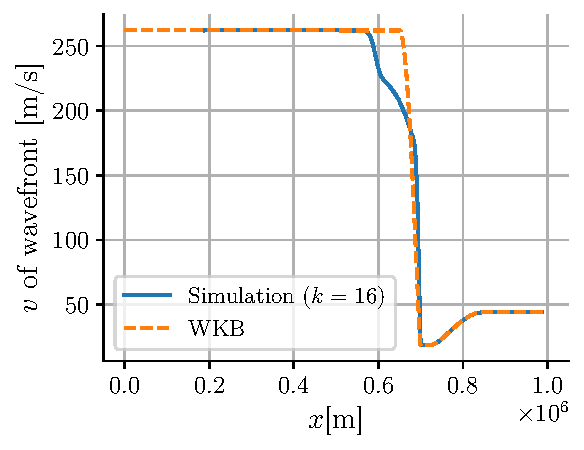
\includegraphics[width=\linewidth]{figures/corail_eq1_vitesse_xa=650000.0.pdf}
        \caption{\(x_a = 650\)km}
        \label{fig:corail_eq1_speed_xa=65km}
    \end{subfigure}
    \caption{Wave properties for \(x_a = 650\)km. Simulated using \(n=8192\) intervals until \hbox{\(t=12000\) \si{\second}}. CFL \(\beta=1\)}
\end{figure}


Let's now analyse what happens when we simulate the system using the wrong although maybe intuitively plausible equation, \autoref{eq:eq2}. The resulting wave can be seen in \autoref{fig:corail_eq2_mouvement}. While the result looks similar at a glance to the result at the begining of this section, we can see that the amplitude of the wave decreases above the reef! Analysing this further using the same methods as described previously, we obtain a plot of the maximal amplitude and speed of the wave peak shown in \autoref{fig:corail_eq2_amplitude}. This time, the simulation undershoots the WKB solution, starting from where the depth changes. The difference between the simulation and the WKB solution remains under 0.02m, which is still quite precise. Like previously howether, the speed matches the WKB solution exactly, as can be seen in \autoref{fig:corail_eq2_vitesse}. The WKB analysis on both equations showed that the speed is the same for both equations, which was verified again here.

\begin{figure}[h]
    \centering
    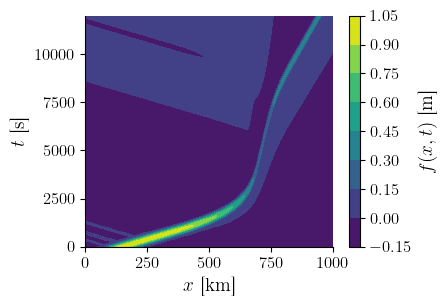
\includegraphics[width=0.6\linewidth]{figures/corail_eq2_mouvement_vague.png}
    \caption{Wave height as a function of space and time, simulated following \autoref{eq:eq2}. Simulated with \(n=16328\) intervals until \(t=12000\). CFL \(\beta=1\)}
    \label{fig:corail_eq2_mouvement}
\end{figure}

\begin{figure}[h]
    \centering
    \begin{subfigure}{0.48\linewidth}
        \centering
        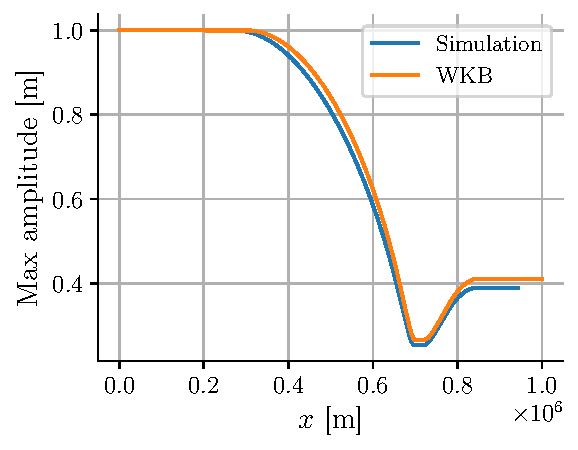
\includegraphics[width=\linewidth]{figures/corail_eq2_amplitude_wkb.pdf}
        \caption{Maximum amplitude reached at each position}
        \label{fig:corail_eq2_amplitude}
    \end{subfigure}
    \begin{subfigure}{0.48\linewidth}
        \centering
        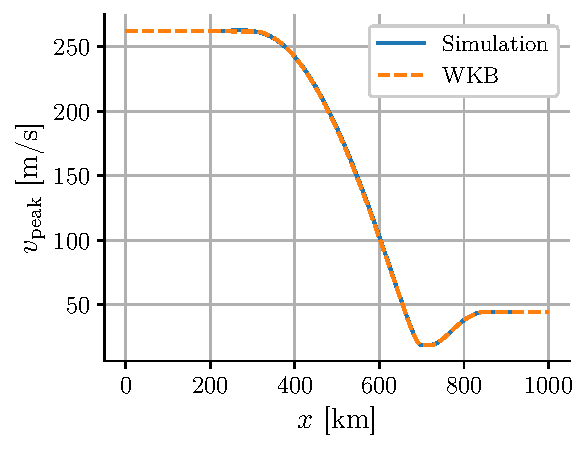
\includegraphics[width=\linewidth]{figures/corail_eq2_vitesse_wkb.pdf}
        \caption{Speed of wave peak}
        \label{fig:corail_eq2_vitesse}
    \end{subfigure}
    \caption{Properties of the wave going towards the coral reef, compared to WKB solution. Simulated w.r.t. \autoref{eq:eq2}, using \(n=8192\) intervals, until \(t=12000\). CFL \(\beta=1\)}
    \label{fig:corail_eq2_properties}
\end{figure}
